\vspace{10pt}

{\centering\subsection*{韩念秋:我学会了包粽子}}

\addcontentsline{toc}{subsection}{韩念秋:我学会了包粽子}

\renewcommand{\leftmark}{韩念秋:我学会了包粽子}

\begin{figure}[htbp]

\centering

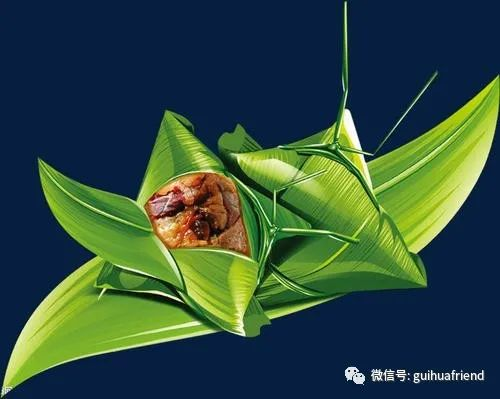
\includegraphics[width = .5\textwidth]{./ch/23.jpg}

\end{figure}





每到端午节的时候,只有我的奶奶和我妈妈在包粽子,我想为他们减轻负担。

先准备一些糯米,红枣,粽叶,五彩线。按着按按照妈妈的指示,我把粽叶围成了一个三角形,把粽子馅儿填到里面。结果做失败了,我很失落,但是妈妈鼓励了我,使我变得自信了。我继续做,做了五六次,最后一次,我满眼充满着期望,那一次我终于做成功了。我拿出五彩线把粽子捆得很严实,粽子一个一个的接着包,我终于忙完了,包完的粽子被我拿到锅里蒸。

打开锅一看,粽子们无忧无虑的躺在那里呢!我把粽叶剥开,就闻到了香喷喷的味道,想必这粽子一定很好吃,中间还有一个很红的红枣在微笑,如同一位可爱的姑娘似的,我用舌头舔了一下,甜中还带着香味,一口下去那粽子,软软糯糯的,真是回味无穷啊!

学包粽子的过程中,我明白做一件事情要坚持到底,才能成功。





\vspace{10pt}



作者:四(1)班 韩念秋



指导老师:周瑞



投稿:2021年5月14日



发表:2021年5月17日














                



\vspace{10pt}

\hline



